\chapter{Scenarios Overview}
\label{ch:scenarios}
% ##################################################################################################################

\hfill \textbf{Authors:} Marcel Rieser, Andreas Horni, Kai Nagel

\begin{center} 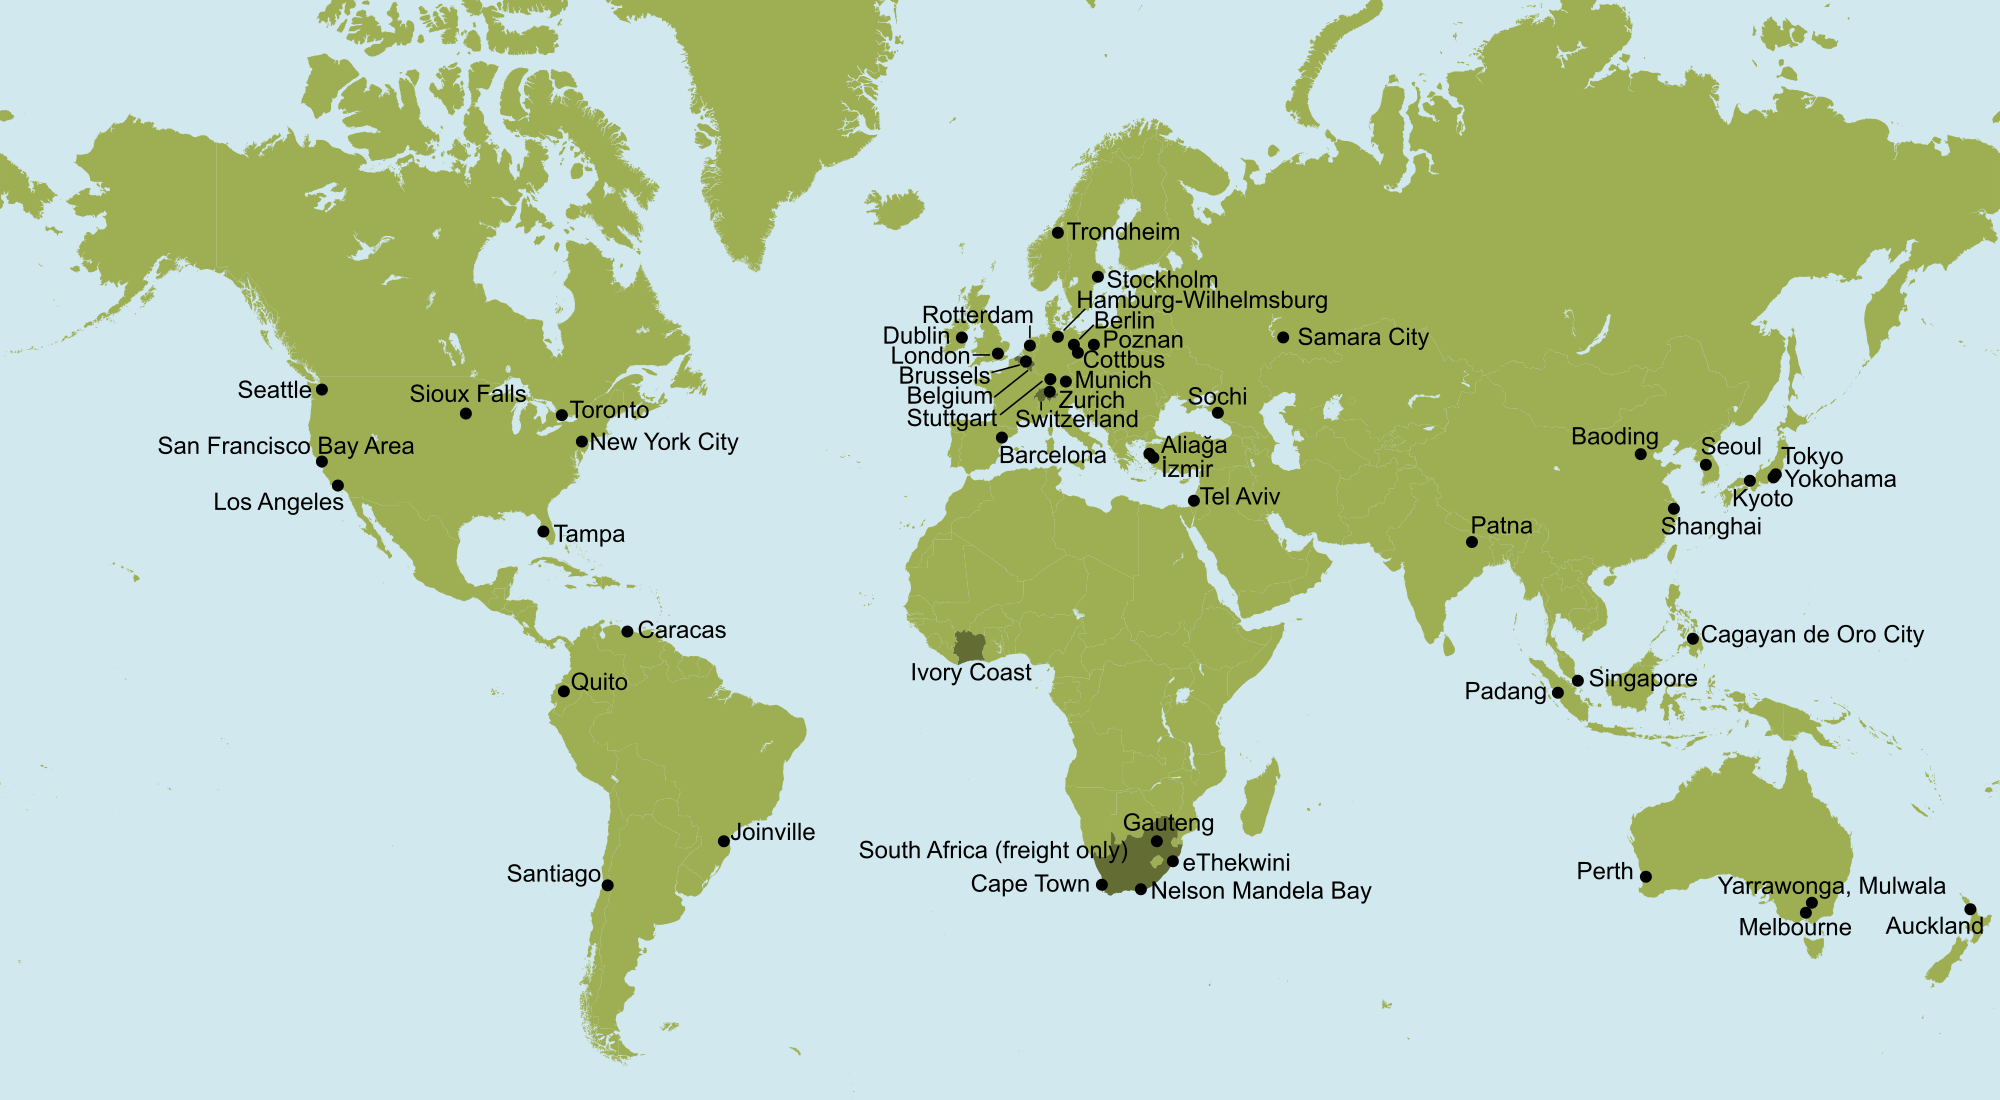
\includegraphics[width=0.7\textwidth, angle=0]{./scenarios/figures/MATSimModelsMap} \end{center}

\editdone{This text has undergone the professional edit. Please no grammatical changes anymore! They are most-probably wrong.}

% ##################################################################################################################
This last book part summarizes \gls{matsim} scenarios, as located on the map in Figure~\ref{fig:scenarios} and listed at \citet[][]{MATSIM-Scenarios_Webpage_2015}).

Many scenarios are not public, due to data privacy issues. However, knowing about general methods and approaches adapted for scenario creation and understanding problems faced during these processes might significantly support and encourage the building of new scenarios. Content basically covers information on study area, population and demand generation, activity locations, network, simulated modes, calibration and validation, achieved results and associated projects. Further subjects involve where to find more information and where/when emphasis is put on certain scenario specialties---be it parsimonious data usage procedures, special modules used, or special modes simulated (such as the parataxis in the Gauteng scenario). Some scenarios have been used for years, with ongoing further development. We target the latest version when reporting. 

Different levels of \gls{matsim} involvement are possible. For some regions and projects, \gls{matsim} is, for example, used only for traffic assignment, where for others, the complete demand is endogenously handled. Couplings with other forecasting models for transport demand generation have been successfully applied, like the coupling with \gls{tasha} for Toronto, or the combination of \gls{matsim} with the Tel Aviv activity-based transport model.

\createfigure%
{Scenarios overview}%
{Scenarios overview}%
{\label{fig:scenarios}}%
{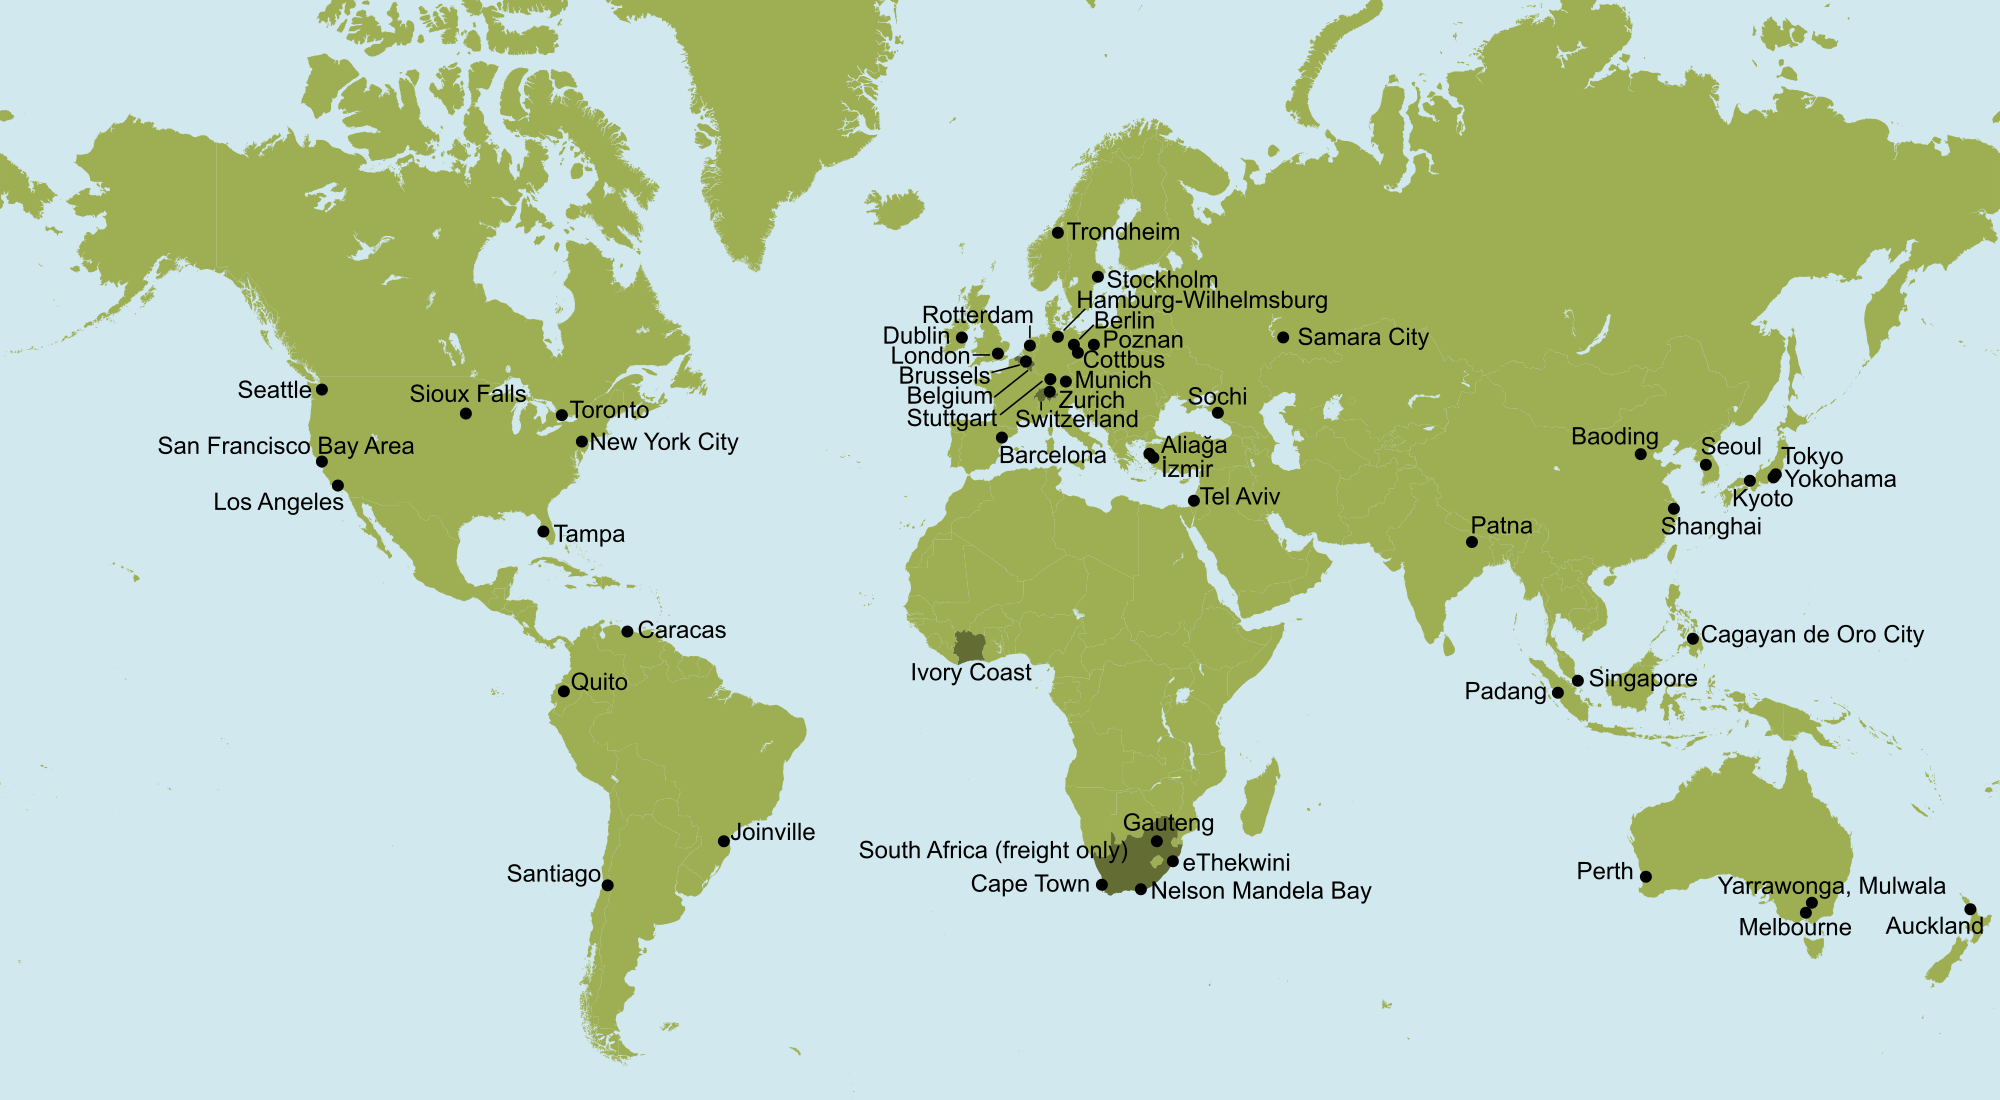
\includegraphics[width=0.99\textwidth, angle=0]{./scenarios/figures/MATSimModelsMap}}%
{}

% ==================================================================================================================
%Further models are available or currently being developed \citep[][]{Axhausen_unpub_Hong_Kong_2013, MATSIM-T-Scenarios_Webpage_2014}: 
% Izmir, 'yalcin.alver@ege.edu.tr'; 'mmetinm@gmail.com' 
% San Francisco Bay Area (alexeip@berkeley.edu) Somewhen given up asking.
% Tampa (sgurram@mail.usf.edu) Somewhen given up asking.
% Ivory Coast (Zilske), 
% LA (Balmer, unfinished), 
% Kyoto (who?)
% Santiago (who?)
% all contacted, where author known.

% ##################################################################################################################
%\section{Discussion and TODOs}
%Will be commented, when chapter is finished. Make final results traceable.

%\ah{
%- region description (characteristics, stats, ...)
%- population (popgen, Balmi plug together)
%- facilities
%- network
%- utility function (estimated, how derived)
%- pt (simulated, pseudo pt)
%- modes
%- freight (siehe keynotes Kai)
%- border crossers/boundary effects
%
%data sources
%methods applied
%
%- special problems faced \& solutions found
%
%- simulation quality
%- calibration \& validation (+available data)
%
%- purpose and sponsor/client
%- associated projects -> see Section \ref{sec:projects}
%
%- specialties: parataxis in Gauteng, connections to other sims (Toronto, Tel-Aviv)
%}

% ##################################################################################################################
